\documentclass[11pt,a4paper]{article}
\usepackage[utf8]{inputenc}
\usepackage[T1]{fontenc}
\usepackage[french]{babel}
\usepackage{graphicx}
\usepackage{amsmath,amssymb}
\usepackage{geometry}
\usepackage{listings}
\usepackage{xcolor}
\usepackage{hyperref}

\geometry{margin=2.5cm}

\lstset{
  basicstyle=\ttfamily\small,
  keywordstyle=\color{blue},
  commentstyle=\color{gray},
  stringstyle=\color{orange},
  breaklines=true,
  frame=single,
  numbers=left,
  numberstyle=\tiny
}

\title{Implémentation de l'algorithme des k-moyennes \\ \large (from scratch en Python)}
\author{[Ton nom]}
\date{\today}

\begin{document}
\maketitle

\section{Introduction}
Le clustering est une tâche d'apprentissage non supervisé qui consiste à regrouper des données similaires. L'algorithme des \emph{k-moyennes} (k-means), introduit par MacQueen (1967) et popularisé par Lloyd (1982), est l'une des méthodes les plus utilisées. L'objectif de ce TP est de l'implémenter \emph{from scratch} en Python, sans utiliser la fonction \texttt{sklearn.cluster.KMeans}, puis d'évaluer son comportement.

\section{Théorie}
\subsection{Principe}
Étant donné un ensemble de points $X = \{x_1, \dots, x_n\} \subset \mathbb{R}^d$ et un entier $k$, on cherche à partitionner $X$ en $k$ groupes $C_1, \dots, C_k$ minimisant l'inertie intra-cluster :
\[
J = \sum_{j=1}^{k} \sum_{x \in C_j} \| x - \mu_j \|^2,
\quad \mu_j = \frac{1}{|C_j|} \sum_{x \in C_j} x.
\]

\subsection{Algorithme de Lloyd}
\begin{enumerate}
  \item Initialiser les $k$ centroïdes.
  \item \textbf{Assignation} : chaque point est affecté au centroïde le plus proche.
  \item \textbf{Mise à jour} : chaque centroïde devient la moyenne de son cluster.
  \item Répéter 2--3 jusqu'à convergence (déplacement des centres $< \varepsilon$ ou nombre max d'itérations).
\end{enumerate}

\subsection{Initialisation k-means++}
Pour éviter les mauvais minima locaux, on choisit les centres initiaux selon Arthur \& Vassilvitskii (2007) : le premier au hasard, puis chaque nouveau centre est tiré avec une probabilité proportionnelle au carré de sa distance au centre le plus proche.

\subsection{Complexité}
Chaque itération coûte $O(n \cdot k \cdot d)$. La convergence est garantie en un nombre fini d'itérations (l'inertie décroît strictement).

\section{Implémentation}
Le code est disponible sur GitHub : \url{https://github.com/[ton-user]/kmeans-from-scratch}.

\subsection{Choix techniques}
\begin{itemize}
  \item \textbf{NumPy} uniquement pour l'algorithme (calcul vectorisé des distances).
  \item \textbf{Initialisation} : k-means++ par défaut, Forgy en option.
  \item \textbf{Critère d'arrêt} : déplacement des centroïdes inférieur à $10^{-6}$ ou 300 itérations.
  \item \textbf{Clusters vides} : réinitialisation aléatoire du centroïde concerné.
\end{itemize}

\subsection{Extrait de code}
\begin{lstlisting}[language=Python]
def _assign(X, centroids):
    d2 = np.sum((X[:, None, :] - centroids[None, :, :]) ** 2, axis=2)
    return np.argmin(d2, axis=1)
\end{lstlisting}

\section{Résultats}
\subsection{Jeu de données}
On génère 500 points synthétiques en 2D répartis en 3 amas gaussiens.

\begin{figure}[h]
  \centering
  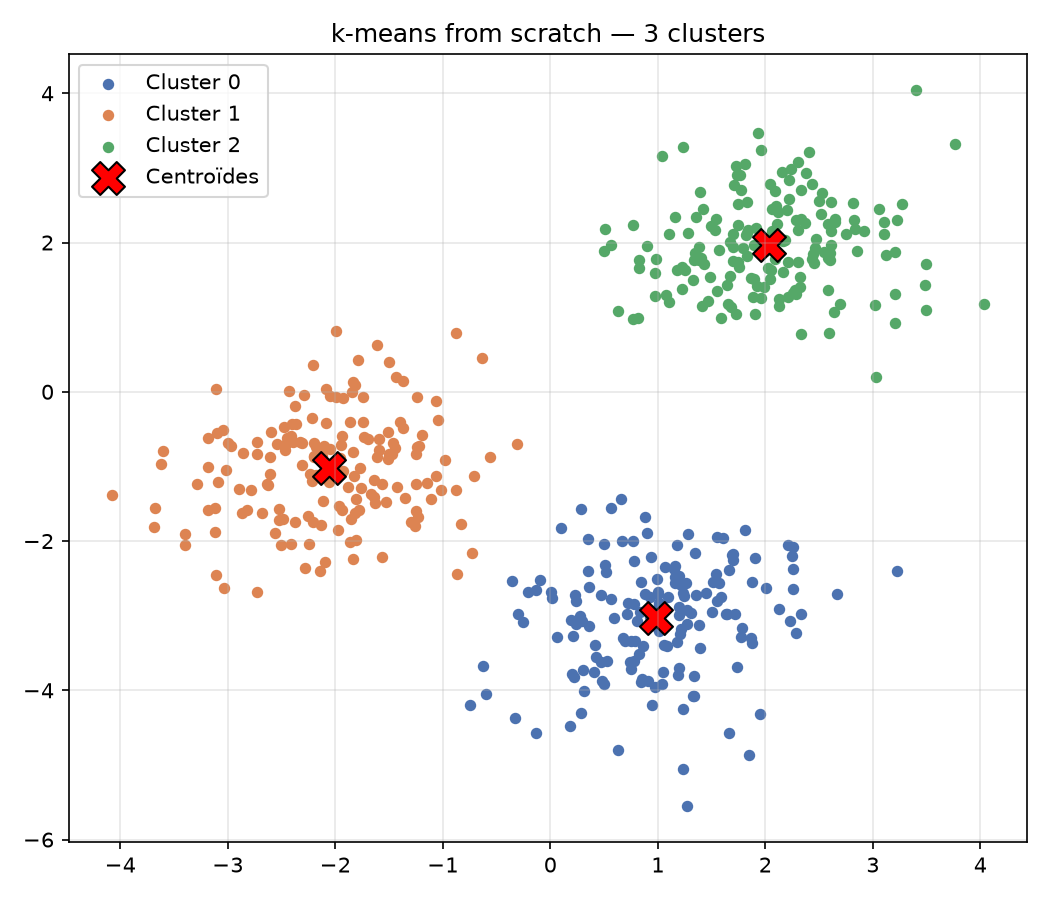
\includegraphics[width=0.7\linewidth]{figures/clustering.png}
  \caption{Clustering obtenu avec $k=3$.}
\end{figure}

\subsection{Convergence}
\begin{figure}[h]
  \centering
  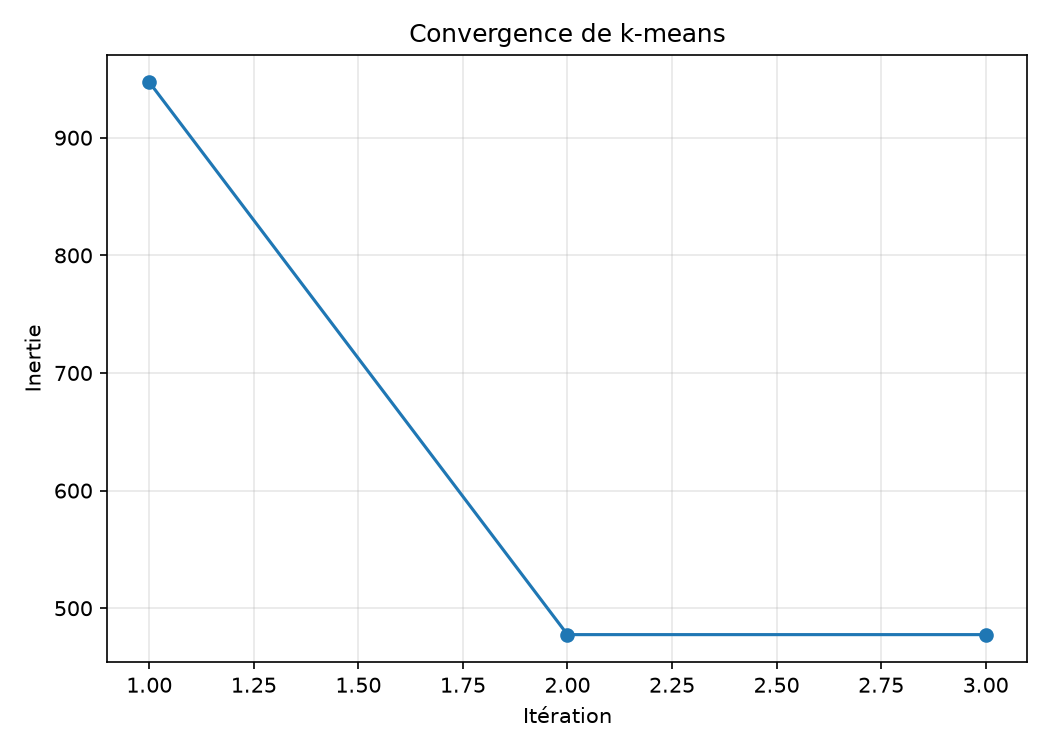
\includegraphics[width=0.7\linewidth]{figures/convergence.png}
  \caption{Décroissance de l'inertie au fil des itérations.}
\end{figure}

\subsection{Choix de $k$ : méthode du coude}
\begin{figure}[h]
  \centering
  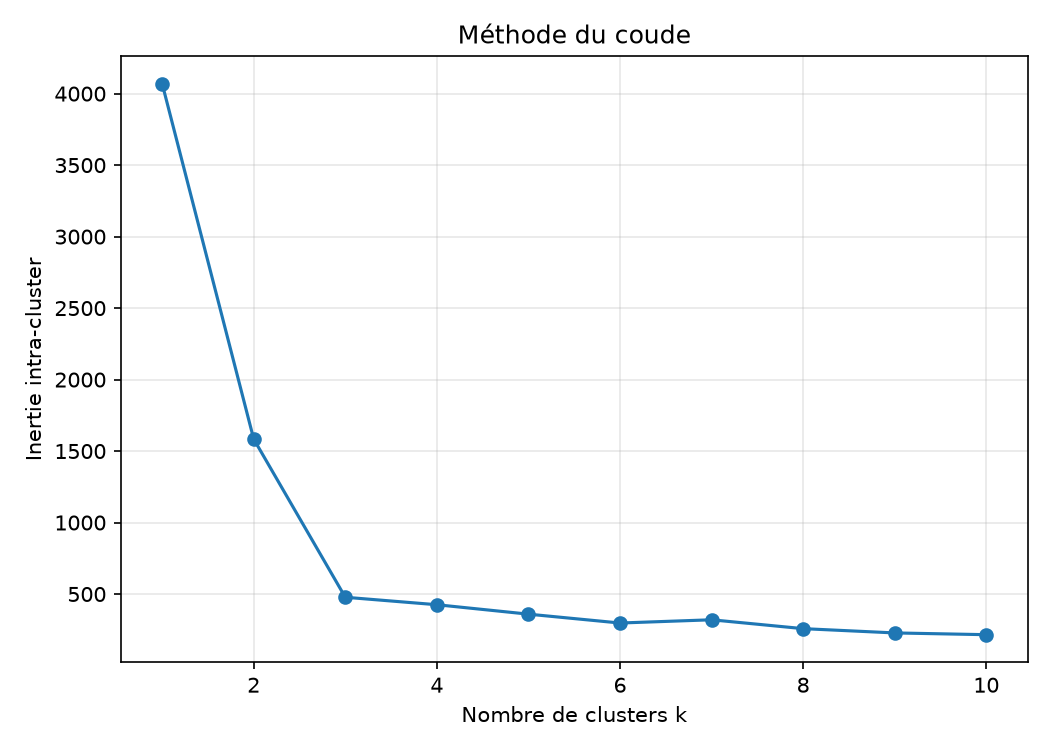
\includegraphics[width=0.7\linewidth]{figures/elbow.png}
  \caption{Inertie en fonction de $k$. Le coude apparaît vers $k=3$.}
\end{figure}

\subsection{Comparaison avec \texttt{sklearn}}
L'inertie finale obtenue est comparable à celle de \texttt{sklearn.cluster.KMeans} (à initialisation équivalente), ce qui valide l'implémentation.

\section{Conclusion}
Nous avons implémenté l'algorithme des k-moyennes from scratch, testé sa convergence et validé ses résultats. Ses limites (sensibilité à l'initialisation, obligation de fixer $k$, hypothèse de clusters sphériques) ont été discutées via la méthode du coude et la comparaison avec une implémentation de référence.

\section*{Références}
\begin{itemize}
  \item MacQueen, J. (1967). \emph{Some methods for classification and analysis of multivariate observations}.
  \item Lloyd, S. (1982). \emph{Least squares quantization in PCM}.
  \item Arthur, D., \& Vassilvitskii, S. (2007). \emph{k-means++: The advantages of careful seeding}.
\end{itemize}

\end{document}